% !Mode:: "TeX::UTF-8"
\documentclass[myposter,portrait]{sciposter}
%% uzitocne package
\usepackage{multicol}
\usepackage{color}
\usepackage{graphicx}
%% znaky s diakritikou
\usepackage[utf8]{inputenc}
\usepackage[T1]{fontenc}
\usepackage[slovak]{babel} % slovenske delenie slov
\usepackage{graphicx}
\usepackage{caption}
\usepackage{fancyvrb}



%% definicia farieb

% \definecolor{mainCol}{rgb}{0.925, 0.941, 0.945} % farba pozadia posteru
\definecolor{mainCol}{rgb}{0.94, 1, 0.92} % farba pozadia posteru
\definecolor{SectionCol}{rgb}{0.98, 1, 0.98} % farba nadpisu
% \definecolor{SectionCol}{rgb}{0.925, 0.941, 0.945} % farba nadpisu
% \definecolor{SectionCol}{rgb}{0.173, 0.243, 0.314} % farba nadpisu
\definecolor{BoxCol}{rgb}{0.18, 0.8, 0.443} % farba boxu okolo nadpisov
\definecolor{TextCol}{rgb}{0.10, 0.24, 0.11} % farba hlavneho textu

\def\mysection#1{
{\color{SectionCol}\section*{\sc\bfseries #1}}}

\usepackage{eso-pic}
\newcommand\BackgroundPic{
\put(0,0){
\parbox[b][\paperheight]{\paperwidth}{%
\vfill
\centering
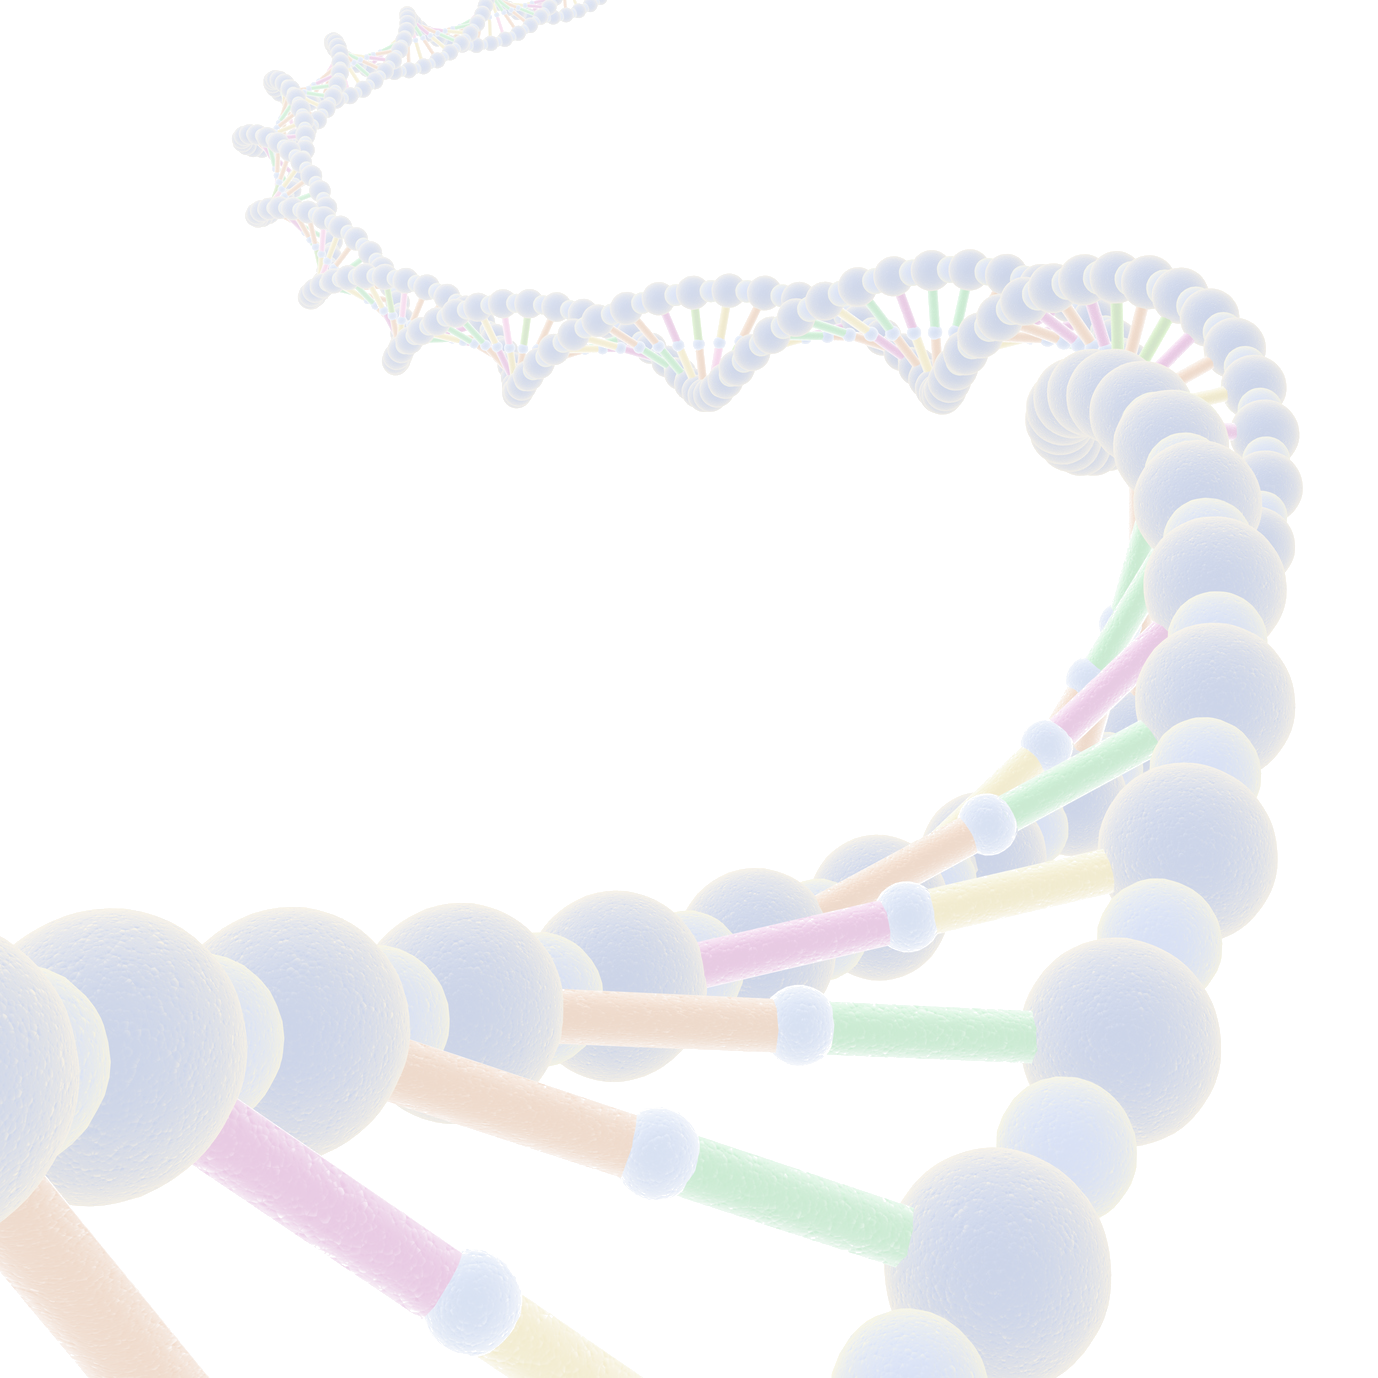
\includegraphics[width=\paperwidth,height=\paperheight]{images/dna_bg}%
\vfill
}}}


\begin{document}
\AddToShipoutPicture{\BackgroundPic}
\setlength{\logowidth}{20cm}
\setlength{\titlewidth}{\textwidth}
\addtolength{\titlewidth}{-\logowidth}
\rightlogo[0.9]{images/fmfilogo-farebne}
\useleftlogofalse

\color{TextCol}
\title{Zarovnávanie sekvencií s~použitím metód klasifikácie}

\author{Michal Hozza\\
  Školiteľ: Tomáš Vinař$^1$, Michal N\'an\'asi$^2$
}
\institute{
$^1$ Katedra aplikovanej informatiky,
FMFI UK, Mlynská dolina, 842~48~Bratislava\\
$^2$ Katedra informatiky,
FMFI UK, Mlynská dolina, 842~48~Bratislava}
\maketitle

\begin{multicols*}{3}


\mysection{Úvod}

Zarovnávanie dvoch DNA sekvencií je jedným zo základných
bioinformatických problémov. Správne zarovnanie identifikuje časti
sekvencie, ktoré vznikli z~toho istého predka (zarovnané bázy), ako aj
inzercie a delécie v~priebehu evolúcie (medzery v~zarovnaní). Obvykle
takéto zarovnanie hľadáme pomocou jednoduchých párových skrytých
Markovovských modelov (pHMM) \cite{durbin}. V~našej práci \cite{hozzaThesis} sa zaoberáme
možnosťami použitia prídavnej informácie o~funkcii vstupných sekvencií
(tzv. anotácie) na zlepšenie kvality takýchto zarovnaní.


\begin{figure}[hbtp]
    \centering
    \begin{BVerbatim}
GTGGACCGTT------CCTTCCGGCAATCACGAGAAAAGCCACGT
GTCGACCGTTTCAGTGACTTGAAGCAATCAGG---AACACCACCT
    \end{BVerbatim}
    \caption{Zarovnanie dvoch sekvencií. V~zarovnaní sa nachádzajú zhody, nezhody a medzery v~oboch sekvenciách}
    \label{fig:alignment_example}
\end{figure}

\mysection{Klasifikácia na základe lokálnej informácie}

Anotácie sme zakomponovali pomocou klasifikátorov, ktoré rozhodujú či dané pozície majú byť zarovnané k~sebe alebo nie. Ako klasifikátor sme použili \emph{náhodný les (angl. Random forest)} \cite{randomForestPaper}, pretože aktuálne patrí medzi najlepšie klasifikátory.

\begin{itemize}
    \item Výstup je hodnota z~intervalu $\left<0,1\right>$, ktorá označuje istotu klasifikátora, že dané dve pozície majú byť zarovnané k~sebe (v~insert stave, že daná pozícia má byť zarovnaná k~medzere).
    \item Atribúty sú okná veľkosti $w$ (obr. \ref{fig:window}), v~ktorých sa nachádza $w$ dvojíc báz v~okolí daných pozícií a ich anotácie (napr. či ide o~gén alebo nie).
\end{itemize}

\begin{figure}
    \centering
    \label{fig:window}
    \subfigure[Match klasifikátor]{%
            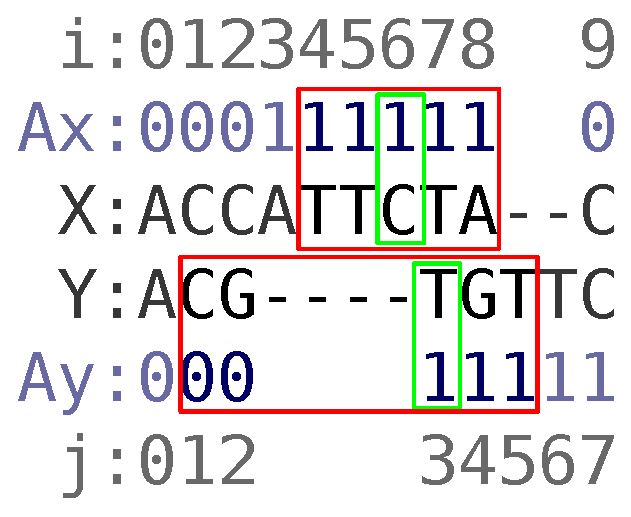
\includegraphics[width=.45\textwidth]{images/window_m}
    }
    % \hspace{0.1\textwidth}
    \subfigure[Indel klasifikátor]{%
            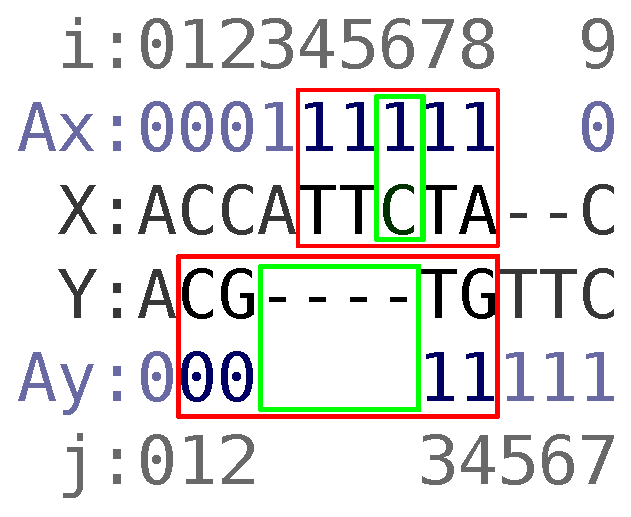
\includegraphics[width=.45\textwidth]{images/window_i}
    }
    \caption{Okno klasifikátora pre pozície $i = 6$ a $j = 3$}
\end{figure}

\begin{itemize}
    \item K~dátam z~okna sme pridali informácie o~zhodách na zodpovedajúcich pozíciách, čím sa nám podarilo vylepšiť úspešnosť klasifikátora.
    \item Úspešnosť Match klasifikátora: \textbf{84,32\%}
    \item Úspešnosť Indel klasifikátora: \textbf{76,46\%}
\end{itemize}

Ukázalo sa teda, že klasifikátor sa dokáže naučiť, ktoré okná majú byť zarovnané k~sebe a ktoré nie (Obr. \ref{fig:clf-dist}).

\begin{figure}
    \centering
    \label{fig:clf-dist}
    \subfigure[Match klasifikátor]{%
            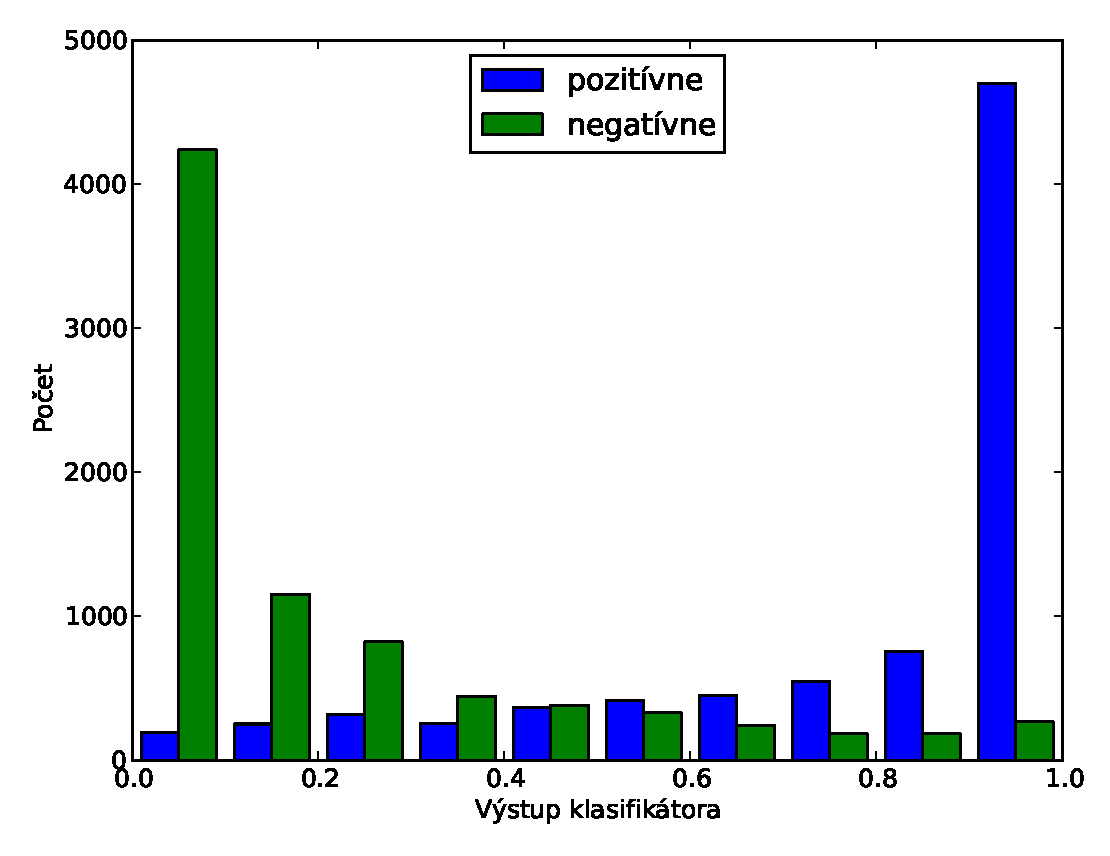
\includegraphics[width=.45\textwidth]{images/randomforest_combined_5_test}
    }
    % \hspace{0.05\textwidth}
    \subfigure[Indel klasifikátor]{%
            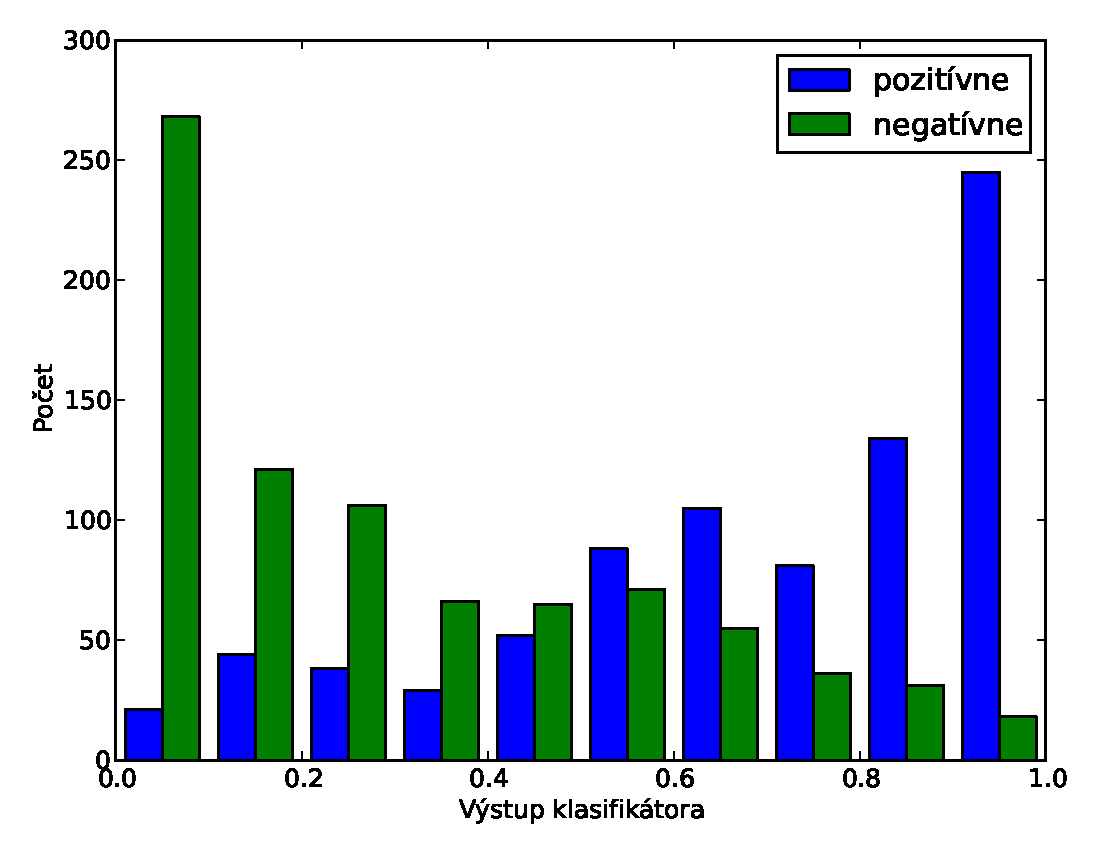
\includegraphics[width=.45\textwidth]{images/randomforest_combined_5_indel_test}
    }
    \caption{Distribúcia výstupu klasifikátora pre pozitívne a negatívne príklady.}
\end{figure}


\begin{figure}
    \centering
    \label{fig:faeture-importances}
    \subfigure[Match klasifikátor]{%
            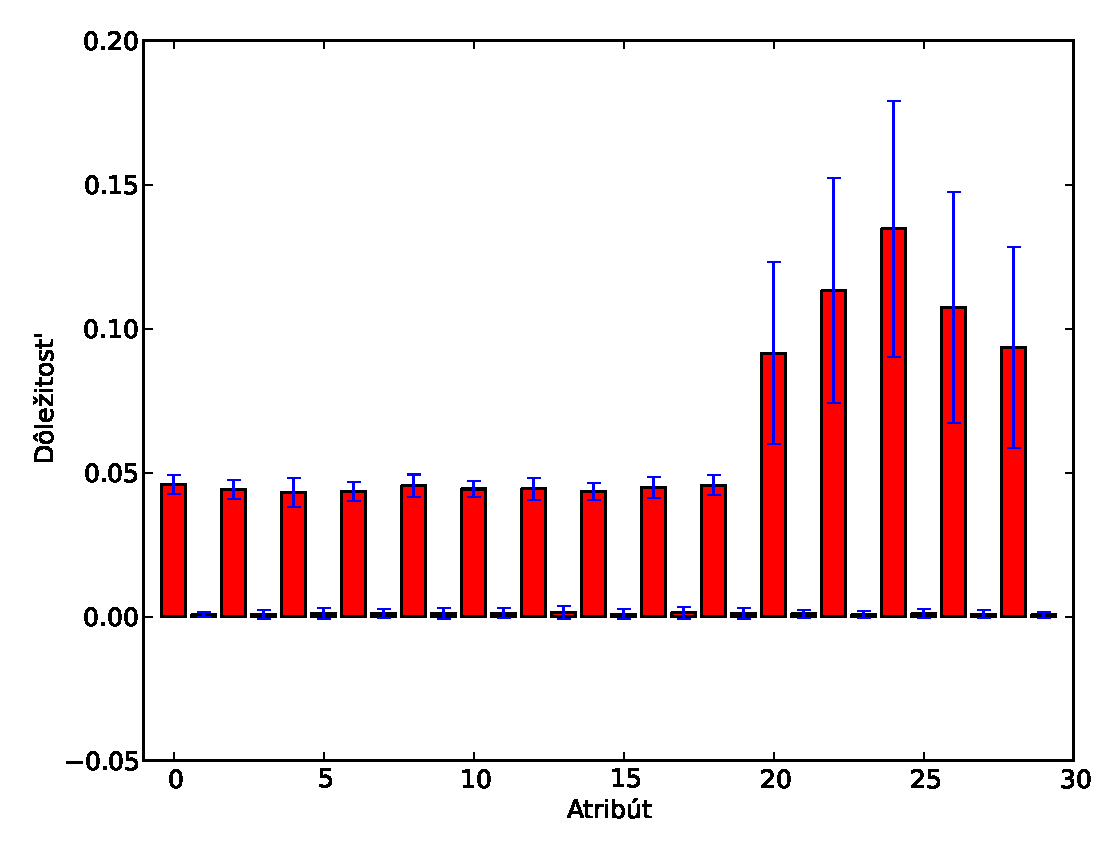
\includegraphics[width=.45\textwidth]{images/randomforest_combined_5_bars}
    }
    % \hspace{0.05\textwidth}
    \subfigure[Indel klasifikátor]{%
            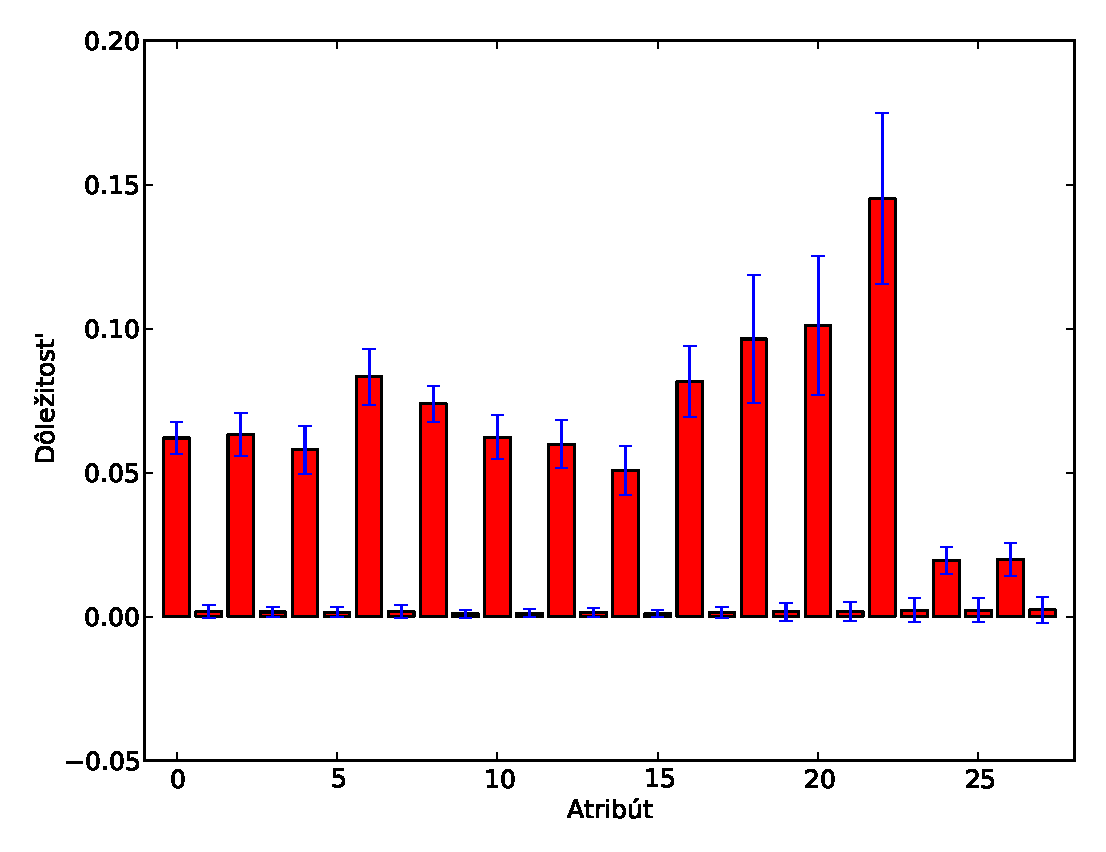
\includegraphics[width=.45\textwidth]{images/randomforest_combined_5_indel_bars}
    }
    \caption{Dôležitosť atribútov v~klasifikátore. Na párnych pozíciach sú bázy, na nepárnych anotácia. Prvých 10 atribútov zodpovedá oknu v~prvej sekvencii, druhých 10 (resp. 8 v~Indel klasifikátore) zodpovedá oknu v~druhej sekvencii a posledných 10 zodpovedá zhodám na príslušných pozíciách (v~Indel klasifikátore sa namiesto medzery zopakuje báze čo je za ňou)}
\end{figure}

\mysection{Zakomponovanie výsledkov klasifikácie do pHMM}

Vyvinuli sme dva modely pre zarovnanie sekvencií s~anotáciami za pomoci klasifikátora, ktoré sú založené na párových skrytých Markovovských modeloch.

\paragraph{Model s~klasifikátorom ako emisiou (Obr. \ref{fig:model-clf}):}
\begin{itemize}
    \item Emisné tabuľky stavov nahradíme výstupom z~klasifikátora.
    \item Model nie je korektný pravdepodobnostný model, pretože pravdepodobnosti emisií nesčitujú do~1.
    \item Prechodové pravdepodobnosti sme natrénovali zo zarovnaní z~trénovacej vzorky.
\end{itemize}

\paragraph{Model s~klasifikátorovou páskou (Obr. \ref{fig:model-clf-tape}):}

\begin{itemize}
    \item Modelujeme navyše sekvenciu výstupov klasifikátora vo forme pásky.
    \item Trénujeme všetky parametre na trénovacej vzorke zarovnaní obohatenej o~pásku s~výstupmi z~klasifikátora.
\end{itemize}

Keďže stále ide o~párový HMM, pásku si musíme predstaviť ako cestu v~2D tabuľke výstupov klasifikátorov, ktorá sa zhoduje s~cestou zarovnania. Teda ak sa pohneme horizontálne  alebo vertikálne, používame Indel klasifikátor a ak sa pohneme diagonálne, tak použijeme Match klasifikátor.

\begin{figure}
    \centering
    \label{fig:faeture-importances}
    \subfigure[
    Model\\ s~klasifikátorom ako emisiou
    ]{%
        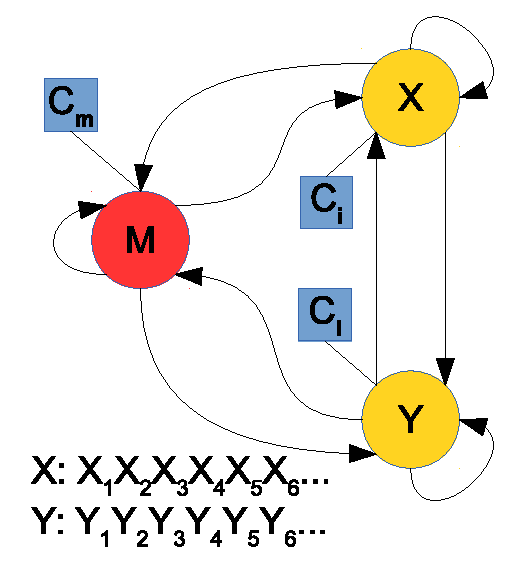
\includegraphics[width=.40\textwidth, clip=true]{images/model_clf}
    }
    \label{fig:model-clf}
    % \hspace{0.05\textwidth}
    \subfigure[
    Model \\s~klasifikátorovou páskou
    ]{%
        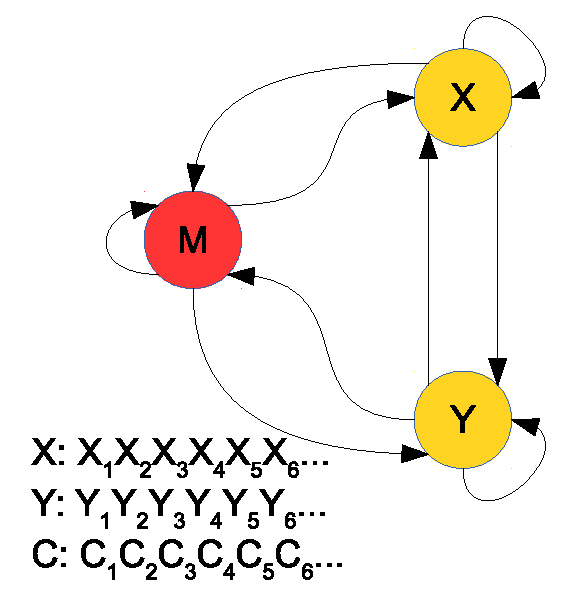
\includegraphics[width=.40\textwidth, clip=true]{images/model_clf_paska}
    }
    \label{fig:model-clf-tape}
    \caption{Modely s~klasifikátorom}
\end{figure}

\mysection{Experimenty}

\begin{table}[htp]
\centering
\begin{tabular}{|l|r@{,}lr@{,}l|r@{,}lr@{,}l|}
\hline
Dáta &  \multicolumn{4}{|c|}{Simulované 1}  & \multicolumn{4}{|c|}{Simulované 2}\\% & \multicolumn{2}{|c|}{Biologické} \\
\hline
Model & \multicolumn{2}{|c}{Zhoda} & \multicolumn{2}{c}{Tranz.} & \multicolumn{2}{|c}{Zhoda} & \multicolumn{2}{c|}{Tranz.}\\% & Zhoda & Tranz.\\
\hline
Ref. model & 85 & 78\% & 61 & 03\% & 6 & 78\% & 8 & 87\%\\% & \% & \%\\
\hline
Model A~& 73 & 95\% & 38 & 10\% & 72 & 62\% & 39 & 48\%\\% & \% & \%\\
\hline
Model A~bez an. & 76 & 07\% & 45 & 63\% &  \multicolumn{2}{|c}{---} & \multicolumn{2}{c|}{---} \\% & \% & \%\\
\hline
Model B & 81 & 62\% & 54 & 94\% & 18 & 57\% & 10 & 50\%\\% & \% & \%\\
\hline
Model B  bez an.& 81 & 22\% & 54 & 18\% & \multicolumn{2}{|c}{---} & \multicolumn{2}{c|}{---}\\% & \% & \%\\
\hline

\end{tabular}
\vspace{0.5cm}
\caption{Porovnanie úspešností modelov. Zhora dole - referenčný model (obyčajný pHMM na zarovnávanie DNA sekvencií), model s~klasifikátorom ako emisiou s~anotáciou a bez nej, model s~klasifikátorovou páskou s~anotáciou a bez nej. Zhoda je počítaná ako percentuálna zhoda originálneho a nového zarovnania. Tranzitivita je počítaná z~troch zarovnaní $AB$, $BC$ a $AC$ ako percentuálna zhoda medzi $AB \circ BC$ a $AC$. Simulované dáta 1 sa snažia napodobňovať biologické procesy, Simulované dáta 2 nezodpovedajú biologickým dátam a sú zložitejšie na natrénovanie pre referenčný model.}
\label{tab:datatype-all}
\end{table}

Experimenty ukázali, že pri jednoduchších dátach bol obyčajný pHMM postačujúci a dosiahol lepšie skóre ako naše modely, ktoré však nezaostávali príliš. Pri zložitejších dátach už obyčajný pHMM nestačil a ukázala sa sila diskriminačného prístupu v~modeli s~klasifikátorom ako emisiou. Taktiež si môžme všimnúť, že pri simulovaných dátach 1 anotácia našim modelom vôbec nepomohla. Pri dátach 2 bola anotácia nutná na správne zarovnanie.

%% zoznam literatury
\bibliographystyle{apalike}
\bibliography{references}

\end{multicols*}
\end{document}

